\documentclass[10pt, compress]{beamer}
\usetheme[titleprogressbar]{m}

\usepackage{booktabs}
\usepackage[scale=2]{ccicons}
\usepackage{minted}

\usepackage{caption}
\captionsetup[figure]{labelformat=empty}
\captionsetup{skip=0pt, belowskip=0pt}

\usepgfplotslibrary{dateplot}

\usemintedstyle{trac}

\title{Poisson Processes and 911 Calls}
\subtitle{}
\date{\today}
\author{Jacob Mortensen}
\institute{Brigham Young University}

\begin{document}
  \maketitle
  
  \section{Introduction}
  \begin{frame}
    \frametitle{Introduction}
    \begin{itemize}
      \item Extreme heat scenarios pose a significant threat to public health
      \item It is of interest for researchers to understand how the effect of heat varies by location
    \end{itemize}
  \end{frame}
  \begin{frame}
    \frametitle{Introduction}
    \centering
    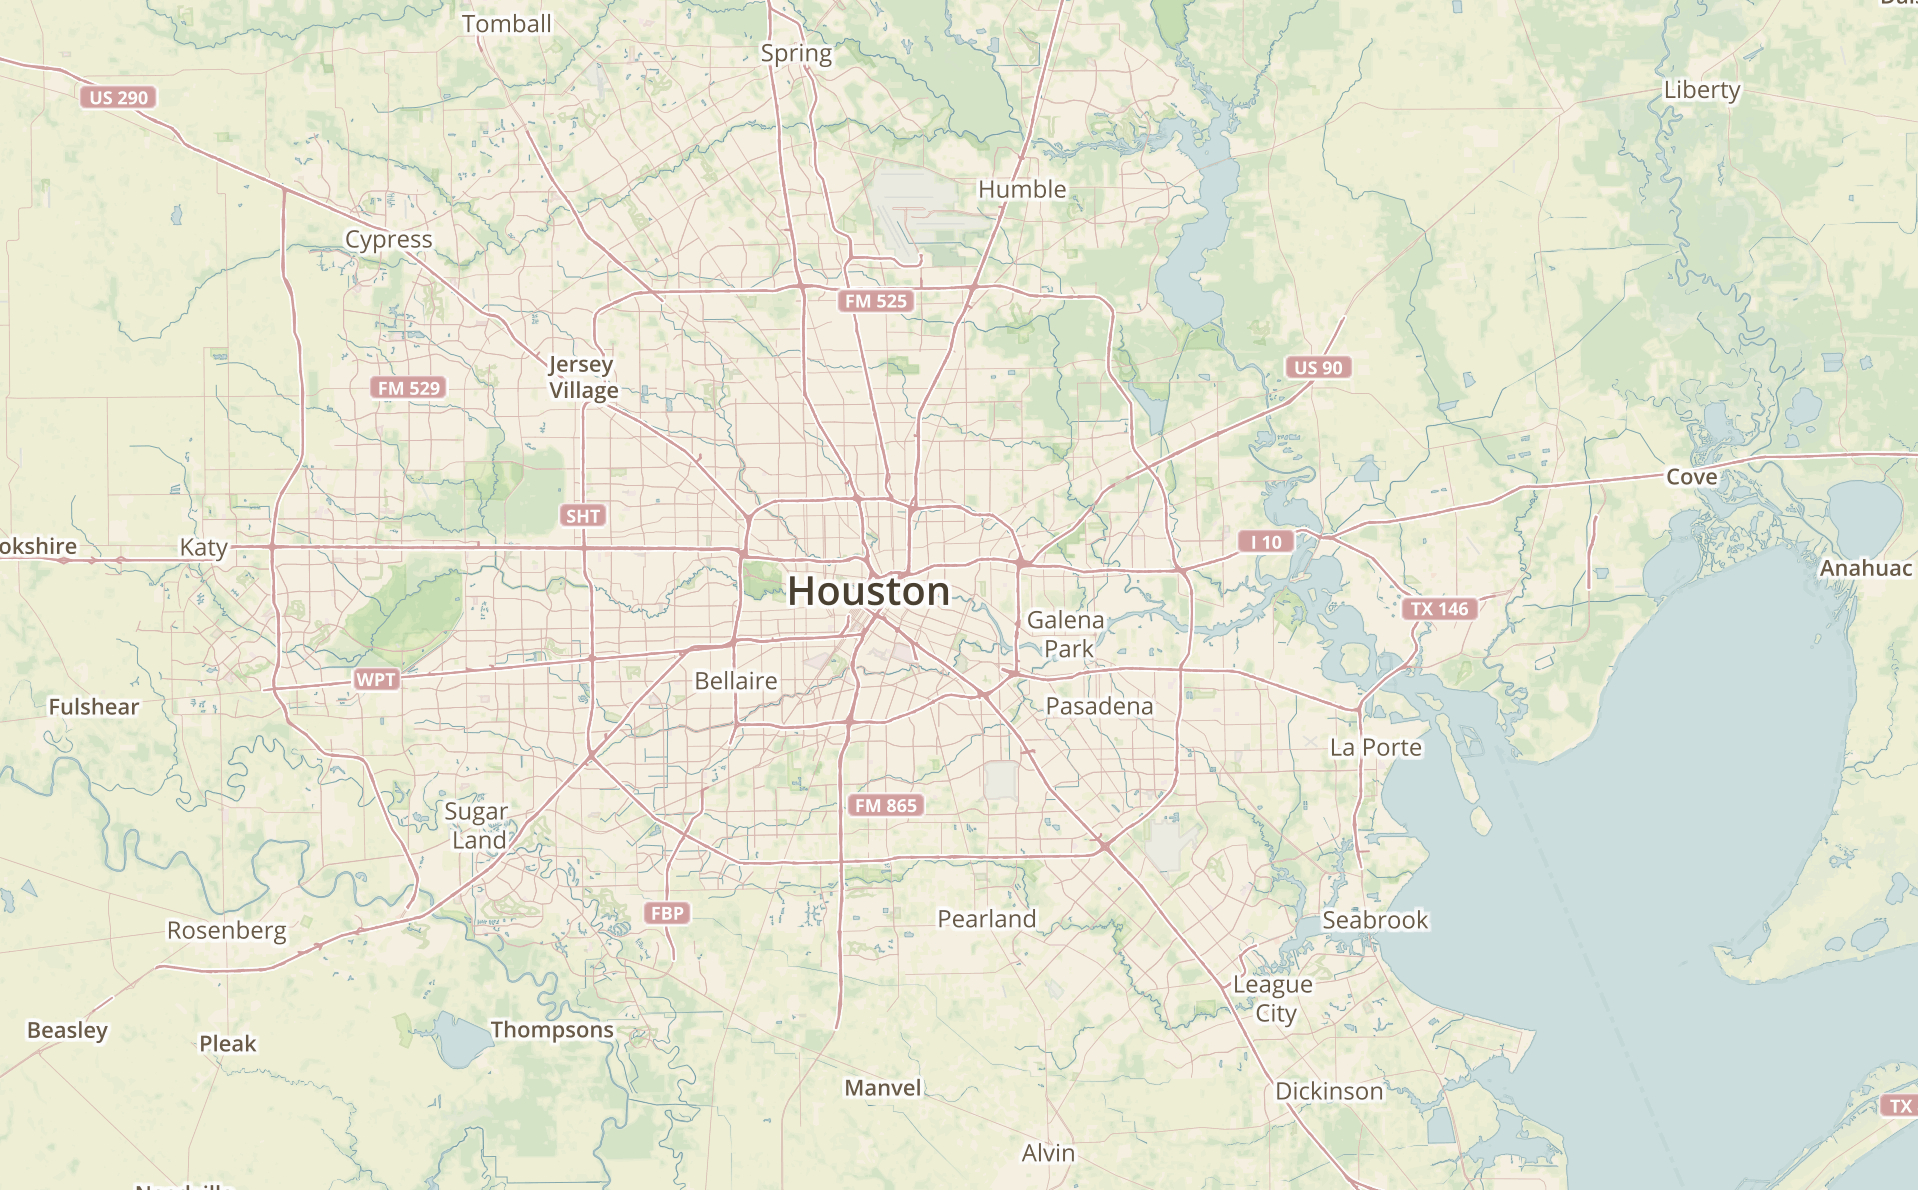
\includegraphics[width=0.8\textwidth]{houston_map.jpg}
  \end{frame}
  \begin{frame}{Introduction}
    \centering
    \begin{minipage}{0.8\textwidth}
      Spatial data is:
      \begin{itemize}
        \item nonlinear
        \item highly correlated
      \end{itemize}
    so how do we model it?
    \end{minipage}
  \end{frame}
  \section{Point Process Models}
  \begin{frame}
    \frametitle{Point Process Models}
    
  \end{frame}
  \section{Poisson Point Processes}

  \section{Our Model}

  
\end{document}
